\section{SECH Hyperbolic Secant Function}

\subsection{Usage}

Computes the hyperbolic secant of the argument.
The syntax for its use is
\begin{verbatim}
   y = sech(x)
\end{verbatim}
\subsection{Function Internals}

The \verb|sech| function is computed from the formula
\[
   \mathrm{sech}(x) = \frac{1}{\cosh(x)}
\]
\subsection{Examples}

Here is a simple plot of the hyperbolic secant function
\begin{verbatim}
--> x = -2*pi:.01:2*pi;
--> plot(x,sech(x)); grid('on');
\end{verbatim}


\centerline{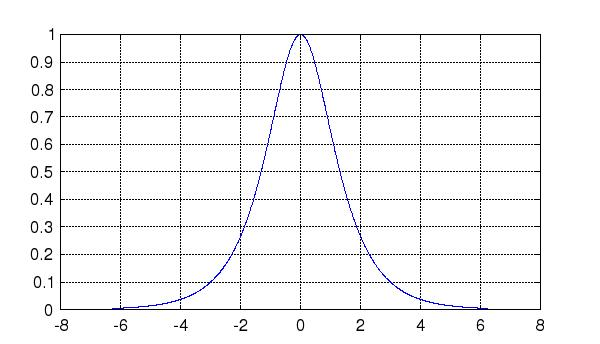
\includegraphics[width=8cm]{sechplot}}

